%The Introduction section clarifies the motivation for the work presented and 
%prepares readers for the structure of the paper.
% context:  orient those readers who are less familiar with your topic and to 
%establish the importance of your work
% need: state the need for your work, as an opposition between what the 
%scientific community currently has and what it wants.
% task: indicate what you have done in an effort to address the need (this is 
%the task)
% object: preview the remainder of the paper to mentally prepare readers for 
%its structure, in the object of the document
%%%%%%%%%%%%%%%%%%%%%%%%%%%%%%%%%%%%%%%%%%%%%%%%%%%%%%%%%%%%%%%%%%%%%%%%%%%%%%%
\section{Introduction}
\label{sec:Introduction}
%%%%%%%%%%%%%%%%%%%%%%%%%%%%%%%%%%%%%%%%%%%%%%%%%%%%%%%%%%%%%%%%%%%%%%%%%%%%%%%

\textbf{From \cite{2012_Liang_BiomedicalOpticalImaging}\\
}The past two decades have witnessed a dramatic growth in biomedical applications of optical microscopy. Mainstream microscopy technologies—including, but not limited to, confocal microscopy, multiphoton microscopy, and optical coherence tomography (OCT)—have greatly benefited from advances in laser technology, fluorescent labeling, scanning mechanisms, and image acquisition; however, all these technologies rely on either optical scattering or fluorescent contrast and have difficulty in sensing optical absorption properties of biological tissues \cite{2010_Hu_Photoacousticimagingand}

Recently, the photoacoustic effect has been utilized for biomedical imaging of tissue optical absorption, leading to a blooming technology—photoacoustic tomography (PAT). In PAT, the object absorbs short-pulsed or intensity-modulated optical irradiation, resulting in heating and further inducing high-frequency ultrasonic waves, which can be detected to map optical absorption.


\textbf{from \cite{2011_Beard_Biomedicalphotoacousticimaging.}:\\}
In essence, a PA image can be regarded as an ultrasound image in which the contrast depends not on the mechanical and elastic properties of the tissue, but its optical properties, speci?cally optical absorption. As a consequence, it offers greater speci?city than conventional ultrasound ima- ging with the ability to detect haemoglobin, lipids, water and other light-absorbing chomophores, but with greater penetration depth than purely optical imaging modalities that rely on ballistic photons. As well as visualizing anatomical structures such as the micro- vasculature, it can also provide functional information in the form of blood oxygenation, blood ?ow and temperature. All of this can be achieved over a wide range of length scales from micrometres to centimetres with scalable spatial resolution. These attributes lend PA imaging to a wide variety of applications in clinical medicine, preclinical research and basic biology for studying cancer, cardiovascular disease, abnormalities of the microcirculation and other conditions. With the emergence of a variety of truly compelling in vivo images obtained by a number of groups around the world in the last 2–3 years, the technique has come of age and the promise of PA imaging is now beginning to be realized. Recent highlights include the demonstration of whole-body small-animal imaging, the ?rst demonstrations of molecular imaging, the introduction of new microscopy modes and the ?rst steps towards clinical breast imaging being taken as well as a myriad of in vivo preclinical imaging studies. In this article, the underlying physical principles of the technique, its practical implementation, and a range of clinical and preclinical applications are reviewed.

\textbf{General about standard microscopy}\\
By magnifying minuscule cellular and subcellular features, optical microscopes provide a powerful tool for studying tissue components and their dynamic interactions. Its excellent imaging contrast in soft tissue has made optical microscopy the most widely used imaging modality in the biomedical community.\cite{2000_Amos_Lessonsfromhistory}  

The visual power of optical microscopy relies on sharp optical focusing. Such power is rapidly reduced as photons travel deeper into biological tissue, a highly scattering medium for electromagnetic waves in the optical spec- tral range. When photons reach the optical diffusion limit ($\approx \unit[1]{mm}$ in tissue), they have typically undergone tens of scattering events, which randomize the photon paths and thus prevent tight focusing~\cite{2000_Fujimoto_Opticalcoherencetomography:}

Although modern optical microscopic techniques have released biologists from the con?nes of ten-micrometer-thick ex vivo tissue slices to a world of volumetric in vivo tissue, optical microscopy is still challenged to image at depths beyond the optical diffusion limit while maintaining high resolution. For decades, engineers have made scant progress by using pure optical approaches to light scattering. 

When a short laser pulse, typically in the nanosecond range, is spatially broadened and then used to irradiate biological tissue, it produces a temperature rise on the order of milli-Kelvin in a short time frame. Consequently, thermoelastic expansion causes emission of acoustic waves, referred to as photoacoustic waves, that can be measured by wideband ultrasonic transducers around the sample. This phenomenon, discovered by Alexander Graham Bell, has been recently exploited for small-animal imaging, because the acquired photoacoustic waves can be combined mathematically to reconstruct the distribution of optical energy absorption. \cite{2005_Ntziachristos_Lookingandlistening}
 
Mesoscopy instead aims to a balance between penetration and resolution with poten- tial applications ranging from imaging structures of a few millimeter dimensions, such as microvasculature, or biological organisms, such as embryos, zebrafish, and drosophila.\cite{2013_Omar_Rasterscanoptoacoustic}  

\textbf{advantages}:
\begin{itemize}
	\item combining ultrasonic-scale spatial resolution with high sensitivity to tissue light absorption
\end{itemize}

\textbf{disadvantages/problems:}
\begin{itemize}
	\item characterized by long acquisition times and is generally not suitable for real time imaging of dynamic processes
\end{itemize}

\textbf{applications (so far for PA tomography}
\begin{itemize}
	\item visualization of the brain structure and lesions, of cerebral hemodynamic responses to hyperoxia and hypoxia and of cerebral cortical responses to neuroactivities induced by whisker stimulations in rats \cite{2003_Wang_Noninvasivelaserinduced}
	\item noninvasive in vivo imaging of exogenous contrast agents in the rat brain using indocyanine green stabilized with polyethylene glycol \cite{2004_Wang_Noninvasivephotoacousticangiography} 
	\item can be applied to different biomedical research areas, including cancer, cardiovascular, immunologic/inflammatory and neurodegenerative diseases
	\item detection of abnormal capillary shapes and sizes can often address rheumatic diseases and systemic inflammatory diseases \cite{2001_ScusselLonzetti_UpdatingAmericanCollege,2006_Cutolo_Nailfoldcapillaroscopyis}
	\item promising tool for vasculature structural imaging,1–3 breast tumor detection,4 epidermal melanin measurement,5,6 and oxygenation monitoring in blood vessels.7, see reference \cite{2006_Li_Improvedinvivo}
	\item In biomedical applications, OA imaging takes advantage of high optical contrast and low acoustic scattering and hence represents a promising tool for breast tumor prediction,2 epidermal melanin measurement,3 and monitoring of oxygenation in blood vessels.4 see references in  \cite{2004_Liao_Optoacousticimagingwith} probably same as \cite{2006_Li_Improvedinvivo}
\end{itemize}

%%%%%%%%%%%%%%%%%%%%%%%%%%%%%%%%%%%%%%%%%%%%%%%%%%%%%%%%%%%%%%%%%%%%%%%%%%%%%%%%
\subsection{Synthetic Aperture}
\label{sec:SyntheticAperture} 


\cite{2012_Ma_Fastscanningcoaxial},

now following from \cite{2004_Liao_Optoacousticimagingwith}:\\
synthetic aperture focusing technique (SAFT) combined with coherence weighting is employed

\begin{figure}[htbp]
	\centering
		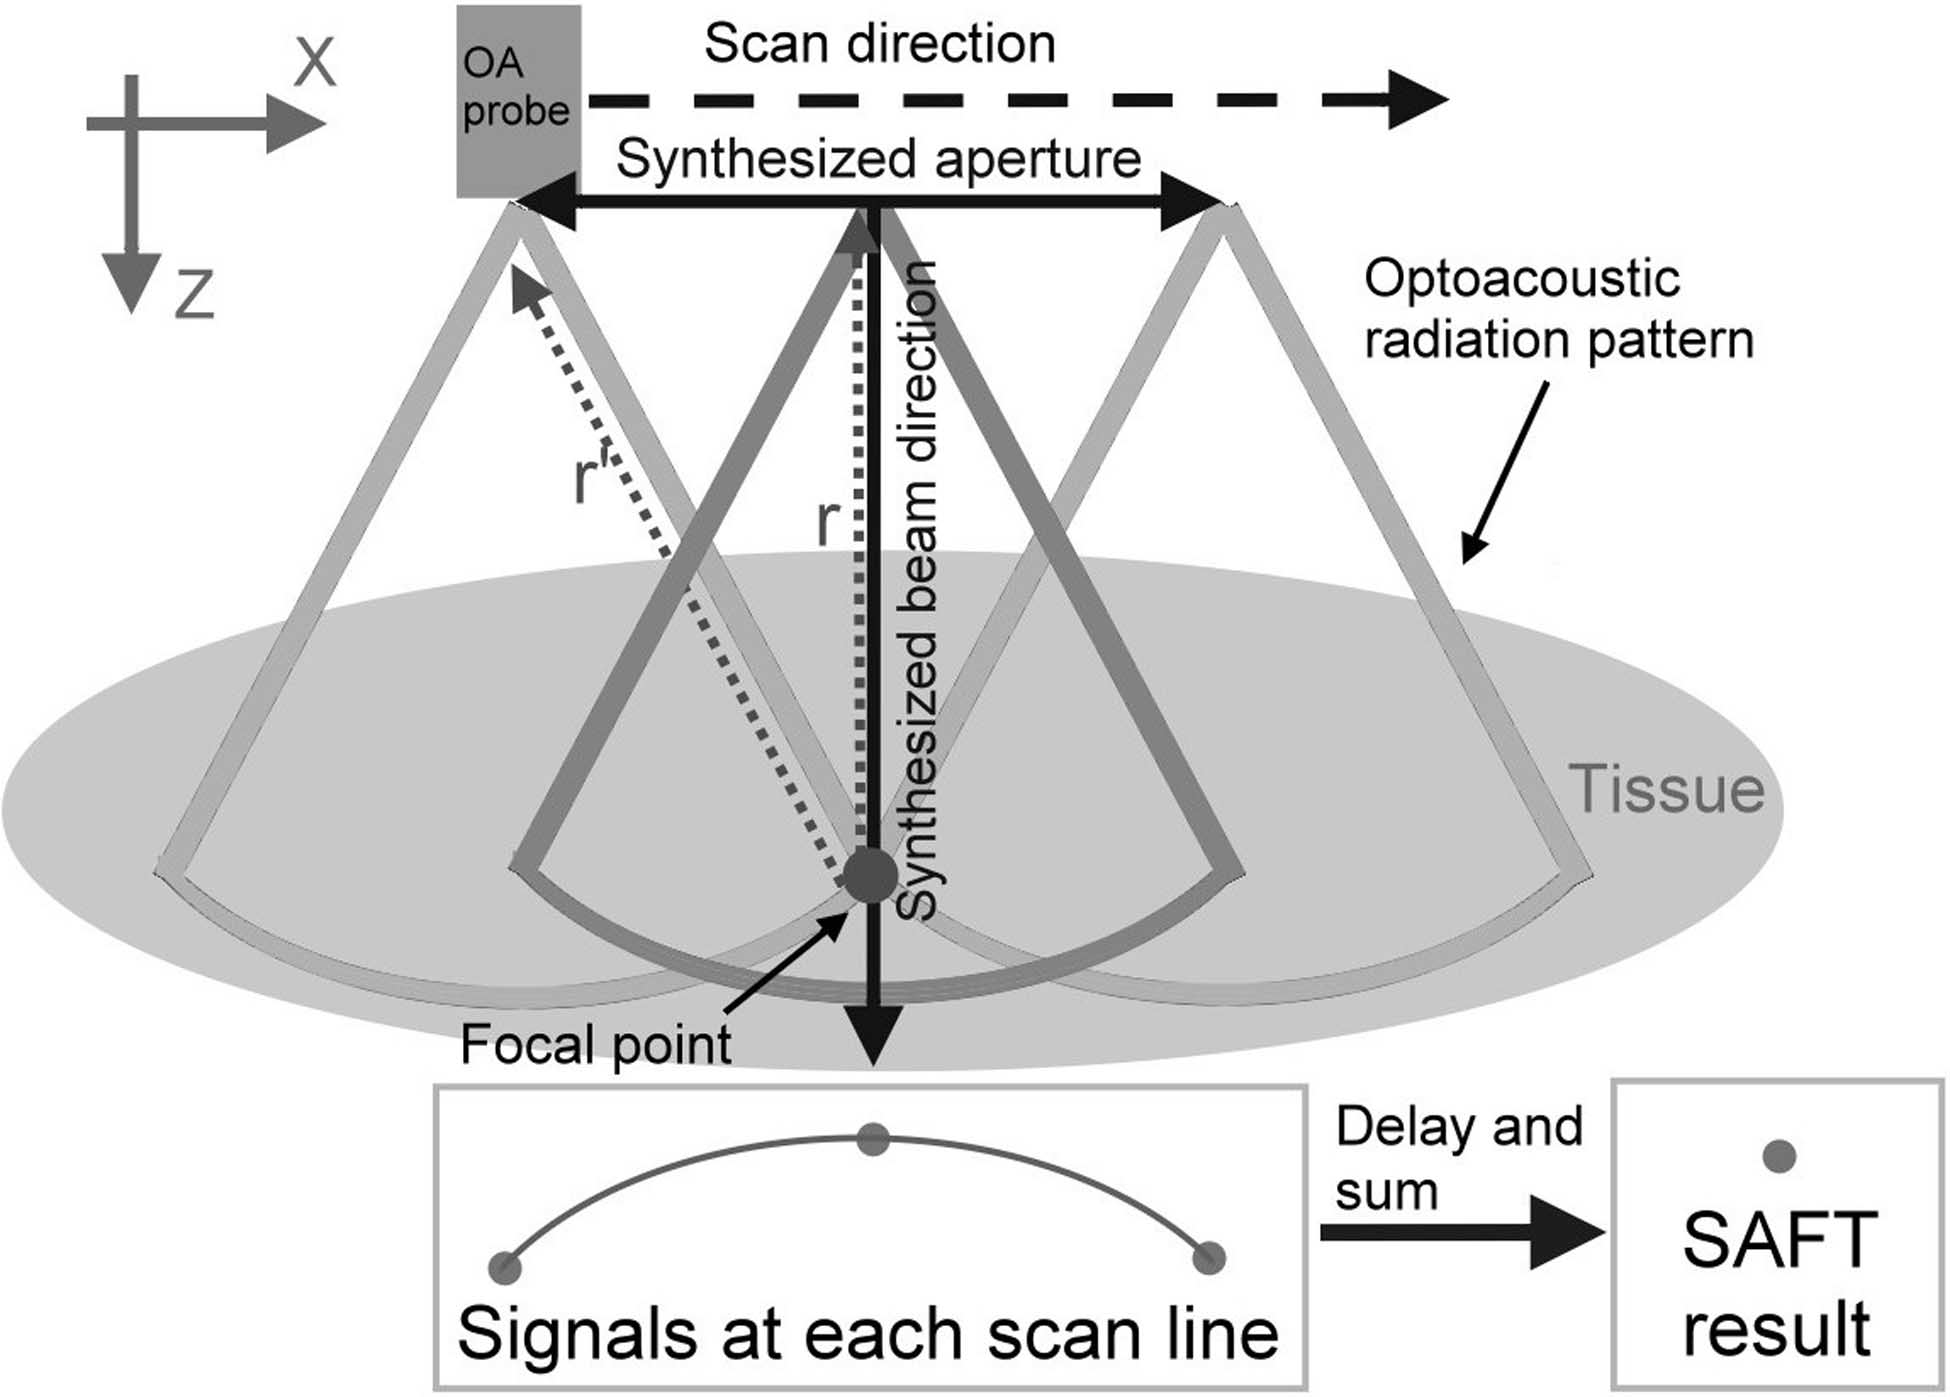
\includegraphics[width=0.50\textwidth]{images/theory/saft_principle.jpg}
	\caption{Graphical illustration of the SAFT technique. \cite{2004_Liao_Optoacousticimagingwith}}
	\label{fig:saft_principle}
\end{figure}
The OA probe is mechanically scanned to acquire a scan line at each scan position. Then the SAFT synthesizes a large aperture by properly delaying and summing the signals received at adjacent scan lines, 
\begin{align}
	RF_\text{SAFT}(t) = \sum_{i=0}^{N-1}{RF(i,t-\Delta t_i})
\end{align}
where $RF_i(t)$ is the received OA signal at the $i$-th position, $\Delta t_i$ is the time delay applied to the signal of scan line $i$, and $N$ denotes the total number of adjacent scan lines included in the SAFT summation. $\Delta t_i$ corresponds to the acoustic propagation time from the synthetic focal point to the OA probe at the $i$-th position. $N$ is determined by the angular extent of the OA radiation pattern, which is the product of the optical illumination pattern and the transducers directivity pattern. A larger extent (i.e., larger $N$) indicates that a bigger OA aperture can be synthesized. In addition to improving the lateral resolution, the SAFT can also increase the signal-to-noise ratio (SNR). Assuming uncorrelated, additive noise (e.g., thermal noise), the SNR improvement is equal to $10 log_{10}(N)$. \cite{2004_Liao_Optoacousticimagingwith}


 











